\chapter{遍历理论}

\section{一个问题}

在正式介绍遍历理论之前，首先看一个利用遍历理论解决概率论问题的例子，以此引入我们将在后续学习的概念.问题是：
\begin{problem}
    考虑数列$x_n=2^{n-1}$，$a_n$表示$x_n$的第一位数字，
    则对$\forall k\in\{1,2,\cdots,9\}$，计算$P(a_n=k) =$?
\end{problem}
\begin{wrapfigure}{l}{0.15\textwidth}
    \vspace{-1.5em}
    \centering
    \renewcommand{\arraystretch}{1.1}
    \setlength{\tabcolsep}{10pt}
    \begin{tabular}{|c|c|c|}
        \hline
        $n$ & $x_n$ & $a_n$ \\
        \hline
        0 & 1 & 1 \\
        \hline
        1 & 2 & 2 \\
        \hline
        2 & 4 & 4 \\
        \hline
        3 & 9 & 9 \\
        \hline
        4 & 16 & 1 \\
        \hline
        5 & 32 & 3 \\
        \hline
    \end{tabular}
    \vspace{-12em}
\end{wrapfigure}\par
\vspace{0.5em}
首先对该问题进行化简，将其解释为可以处理的数学问题.\par
$\begin{aligned}
    x_n=2^n,a_n=x_n\text{的首一数字} &\Leftrightarrow \exists m\in\mathbb{N},\; \text{使得}a_n \cdot 10^m \leqslant 2^n \leqslant (a_n+1) \cdot 10^m \\
    &\xLongleftrightarrow{\text{取对数}}\log{a_n}+m \leqslant n\log{2} \leqslant \log{a_n+1} +m \\
    &\xLongleftrightarrow{\text{取小数部分}} \log{a_n} \leqslant \{n\log{2}\} \leqslant \log{(a_n+1)} \\
    &\Longleftrightarrow \{n\log{2}\} \in [\log{a_n},\log{(a_n+1)}]
\end{aligned}$\par
\vspace{2em}\par\noindent
\begin{itemize*}
    \item $P(a_n=k)=\lim_{N\to\infty}{\frac{\big|\{0 \leqslant n \leqslant N-1|a_n=k\}\big|}{|N|}}=\lim_{N\to\infty}{\frac{1}{N} \left( \sum_{n=0}^{N-1}{\chi_{I_k}\big(\{n\log{2}\}\big)}\right)},\;I_k = [\log{k},\log{(k+1)}]$\par
\end{itemize*}

为了求出上述概率，我们需要引入均匀分布的概念.\par

\begin{definition}{均匀分布}
    设$\{x_n\}_{n\in\mathbb{N}} \subseteq [0,1]$，如果对于任意区间$I \subseteq [0,1]$，$\{x_n\}$落入区间$I$的概率等于$|I|$，即
    \[\lim_{N\to\infty}{\frac{\Big|\big\{1\leqslant n \leqslant N|x_n \in I\big\}\Big|}{N}} = |I|\]
    那么称$\{x_n\}_{n\in\mathbb{N}}$在$[0,1]$中\textbf{均匀分布}.
\end{definition}

下面还有均匀分布的等价刻画.
\begin{proposition}{均匀分布的等价刻画}
    $\{x_n\}_{n\in\mathbb{N}}$在$[0,1]$中均匀分布$\Longleftrightarrow\; \forall\, f\in C([0,1]), f(0)=f(1), \frac{1}{N}\sum_{n=1}^N{f(x_n)}\to \int_{0}^{1}{f(x)}\d x.$
\end{proposition}
\begin{proof}
    \begin{itemize}
        \item[“$\Rightarrow$”] 由均匀分布的定义可知，$\forall\, I \subseteq [0,1]$，$\frac{1}{N}\sum_{n=1}^N{\chi_{I}(x_n)} \to |I| = \int_0^1{\chi_{I}(x)}\d x$.\par
        则对简单函数$\varphi(x)=\sum_{i=1}^n{c_1\chi_{I_1}(x)}$，$\frac{1}{N}\sum_{n=1}^N{\varphi(x_n)}\to \int_{0}^{1}{\varphi(x)}\d x$.\par
        利用简单函数逼近一般可测函数$f(x)$， \par
        即$\forall\, \varepsilon>0,\exists\, \varphi(x)=\sum_{i=1}^n{c_i\chi_{I_i}(x)}$，s.t. $|\varphi(x)-f(x)| < \varepsilon(\forall\, x\in [0,1])$.\par
        故$\left\lvert \frac{1}{N}\sum_{n=1}^N{f(x_n)} - \frac{1}{N}\sum_{n=1}^N{\varphi(x_n)} \right\rvert \leqslant \frac{1}{N}\sum_{n=1}^N{\left\lvert f(x_n)-\varphi(x_n) \right\rvert} < \varepsilon$.\par
        $\Rightarrow \frac{1}{N}\sum_{n=1}^N{\varphi(x_n)} - \varepsilon \leq \frac{1}{N}\sum_{n=1}^N{f(x_n)} \leq \frac{1}{N}\sum_{n=1}^N{\varphi(x_n)} + \varepsilon$.\par
        令$n\to\infty$，取上下极限，其中下面两个不等号成立的原因是积分的绝对值不等式
        \begin{alignat*}{2}
            \int_0^1{\varphi(x)}\d x - \varepsilon &\leq \varliminf_{n\to\infty}{\frac{1}{N}\sum_{n=1}^N{f(x_n)}} \leq \varlimsup_{n\to\infty}{\frac{1}{N}\sum_{n=1}^N{f(x_n)}} &&\leq \int_0^1{\varphi(x)}\d x + \varepsilon  \\
            \int_0^1{f(x)}\d x - 2\varepsilon &\leq &&\leq \int_0^1{f(x)}\d x + 2\varepsilon
        \end{alignat*}
        令$\varepsilon\to 0 \Rightarrow \frac{1}{N}\sum_{n=1}^N{f(x_n)}\to \int_{0}^{1}{f(x)}\d x$.\par
    \end{itemize}
    \begin{minipage}[t]{0.8\textwidth}
    \begin{itemize}
        \item[“$\Leftarrow$"] $\forall\, I \subseteq [0,1]$，构造连续函数列$\{\varphi_n(x)\}_{n\in\mathbb{N}}$和$\{\psi_n(x)\}_{n\in\mathbb{N}}$，使
        \begin{enumerate}[(1)]
            \item $\varphi_n(x) \leq \chi_{I}(x) \leq \psi_n(x)$
            \item $\int_0^1{\varphi_n(x)}\d x \to \int_0^1{\chi_{I}(x)}\d x.$\par
            $\int_0^1{\psi_n(x)}\d x \to \int_0^1{\chi_{I}(x)}\d x.$\par
        \end{enumerate}
        $\Rightarrow \frac{1}{N}\sum_{n=1}^N{\varphi_n(x_n)} \leq \frac{1}{N}\sum_{n=1}^N{\chi_{I}(x_n)} \leq \frac{1}{N}\sum_{n=1}^N{\psi_n(x_n)}$.\par
        $\xLongrightarrow{n\to\infty}\int_0^1{\varphi_n(x)}\d x \leq \varliminf_{n\to\infty}{\sum_{n=1}^N{\chi_{I}(x_n)}} \leq \varlimsup_{n\to\infty}{\sum_{n=1}^N{\chi_{I}(x_n)}} \leq \int_0^1{\psi_n(x)}\d x$.\par
        $\Rightarrow \lim_{n\to\infty}{\sum_{k=1}^N{\chi_{I}(x_k)}} = \int_0^1{\chi_{I}(x)}\d x$.\par
    \end{itemize}
    \end{minipage}
    \begin{minipage}[t]{0.225\textwidth}
        \vspace{0 em}
        
\includegraphics[width=1\textwidth]{fig/2.1.png}
        \captionof{figure}{连续函数逼近特征函数}
    \end{minipage}\par
\end{proof}\par

\begin{itemize}
    \item 上述定理给了我们用连续函数刻画均匀分布的方法，如果我们把连续的条件加强为三阶连续可导，设$f \in C^3([0,1])$，$f(0)=f(1)$，由Fourier分析可知可以对上述函数作Fourier级数展开$f(x)=\frac{a_0}{2}+\sum_{n=1}^\infty(a_n\cos{2\pi nx}+b_n\sin{2\pi nx})\, (\forall\, x\in[0,1])$.并且有以下定理.
\end{itemize}

\begin{theorem*}
    若$f\in C^1([0,1])$，$\frac{a_0}{2}+\sum_{n=1}^N(a_n\cos{2\pi nx}+b_n\sin{2\pi nx})\rightrightarrows f(x) \, (\forall\, x\in[0,1])$.
\end{theorem*}

借由Fourier级数，又可以得到以下使用正余弦和刻画均匀分布的方法.

\begin{theorem}
    $\forall\, f \in C^3([0,1]), f(0)=f(1),\frac{1}{N}\sum_{n=1}^N{f(x_n)}\to \int_{0}^{1}{f(x)}\d x$\par
    $\Leftrightarrow \frac{1}{N}\sum_{k=1}^N{\cos{2\pi kx_n}}\to 0,\frac{1}{N}\sum_{k=1}^N{\sin{2\pi kx_n}}\to 0$.\par
\end{theorem}
\begin{proof}
    \begin{itemize}
        \item[“$\Rightarrow$”] 取$f(x)=\cos{2\pi kx} \Rightarrow \frac{1}{N}\sum_{n=1}^N{\cos{2\pi kx_n}} \to \int_0^1{\cos{2\pi kx}} = 0$.\par
        对$\sin$的情形同理可证.
        \item[“$\Leftarrow$”] $\forall\, f \in C^3([0,1]),f(0)=f(1),\frac{a_0}{2}+\sum_{n=1}^N(a_n\cos{2\pi nx}+b_n\sin{2\pi nx})\rightrightarrows f(x)$\par
        $\Rightarrow \forall\, \varepsilon>0,\exists N,\text{s.t.}\left\lvert f(x) - \left(\frac{a_0}{2}+\sum_{n=1}^N(a_n\cos{2\pi nx}+b_n\sin{2\pi nx})\right)\right\rvert < \varepsilon,\,\forall\, x\in [0,1]$.\par
        记$\varphi_N(x) = \frac{a_0}{2}+\sum_{n=1}^N(a_n\cos{2\pi nx}+b_n\sin{2\pi nx})$\par
        则$\frac{1}{L}\sum_{i=1}^L{\varphi_N(x_n)} - \varepsilon \leq \frac{1}{L}\sum_{i=1}^L{f(x_n)} \leq \frac{1}{L}\sum_{i=1}^L{\varphi_N(x_n)} + \varepsilon$.\par
        令$L\to\infty$，则$\lim_{L\to\infty}\frac{1}{L}\sum_{i=1}^L{\varphi_N(x_n)}=\lim_{L\to\infty}{\frac{1}{L}\sum_{i=1}^L{\left(\frac{a_0}{2}+\sum_{n=1}^N(a_n\cos{2\pi nx}+b_n\sin{2\pi nx})\right)}}=\frac{a_0}{2}=\int_0^1{f(x)}\d x$.\par
        故上述不等式变为$\int_0^1{f(x)}\d x-\varepsilon \leq \varliminf_{n\to\infty}{\frac{1}{N}\sum_{n=1}^N{f(x_n)}} \leq \varlimsup_{n\to\infty}{\frac{1}{N}\sum_{n=1}^N{f(x_n)}} \leq \int_0^1{f(x)}\d x+\varepsilon$.\par
        再令$\varepsilon\to 0 \Rightarrow \frac{1}{N}\sum_{n=1}^N{f(x_n)}\to \int_{0}^{1}{f(x)}\d x$
    \end{itemize}
\end{proof}\par\noindent

\begin{itemize}
    \item 有了上述定理的准备，下一步要说明的是$\big\{\{n\log{2}\}\big\}_{n\in\mathbb{N}}$在$[0,1]$中均匀分布.\par
    \begin{proof}
        $\forall\, k \in \mathbb{N}$，考虑$\left| \frac{1}{N}\sum_{n=1}^{N-1}\cos \left(k\cdot\{n\log{2}\}2\pi\right) \right|$.\par
        由于添加整数对于$\cos \left(k\cdot\{n\log{2}\}2\pi\right)$的值没有影响，因此
        \begin{align*}
            \left| \frac{1}{N}\sum_{n=1}^{N-1}\cos \left(k\cdot\{n\log{2}\}2\pi\right) \right| &= \left| \frac{1}{N}\sum_{n=1}^{N-1}\cos \left(k\cdot n\log{2}\cdot 2\pi\right) \right| \\
            &= \left| \frac{1}{N}\sum_{n=0}^{N-1}{\frac{2\cos \left(k\cdot n\log{2}\cdot 2\pi\right)\sin \left(\log{2}\cdot k\pi\right)}{2\sin \left(\log{2}\cdot k\pi\right)}} \right| \\
            &\xlongequal{\text{积化和差}} \left|\frac{1}{N}\sum_{n=0}^{N-1}{\frac{\sin \left(\log{2}\cdot(2n+1)k\pi\right) - \sin \left(\log{2}\cdot(2n-1)k\pi\right)}{2\sin \left(\log{2}\cdot k\pi\right)}}\right| \\
            &= \left|\frac{1}{N}\frac{\sin \left(\log{2}\cdot(2N-1)k\pi\right) - \sin \left(\log{2}\cdot(-k\pi)\right)}{2\sin \left(\log{2}\cdot k\pi\right)}\right| \\
            &\leq \frac{1}{N}\frac{1}{\left|\sin \left(\log{2}\cdot k\pi\right)\right|} \to 0\,(N\to\infty)
        \end{align*}
        对$\sin$同理.
    \end{proof}
    \item $x_n=2^n,a_n=x_n\text{的首一数字}$，由于$\{n\log{2}\}$在$[0,1]$中均匀分布，因此\par
    $P(a_n=k)=\lim_{N\to\infty}{\frac{1}{N}\sum_{n=0}^N{\chi_{I_k}\big(\{n\log{2}\}\big)}} = \int_0^1{\chi_{I_k}(x)}\d x = \log{\left(1+\frac{1}{k}\right)} \, I_k=[\log{k},\log{(k+1)}]$.\par
    \item 这个结果就是大名鼎鼎的\bluebf{本$\cdot$福特定理}
\end{itemize}

在上面一系列的证明过程中，最重要的部分是对$\frac{1}{L}\sum_{n=1}^L{f(x)}$的估计，关于这个估计，我们先不加证明的引入以下定理：
\begin{theorem}{Birkhoff遍历定理}
    设$(X,\mathcal{B},m)$是一个概率测度空间，$T:(X,\mathcal{B},m)\to(X,\mathcal{B},m)$是一个保测遍历映射，那么$\forall\, f \in L^1(X,\mathcal{B},m)$，$\frac{1}{N}\sum_{n=0}^{N-1}{f(T^n(x))} \to \int_X{f}\d m\; \aew x$.
\end{theorem}
该定理包含的保测映射、遍历映射等概念将在后续学习中一一提及.

\section{保测映射}

\begin{definition}{保测映射}
    设$(X,\mathcal{B},m)$是一个概率测度空间，$T:(X,\mathcal{B}) \to (X,\mathcal{B})$是一个\textbf{可测映射}(可测集的原像是可测集).
    \begin{itemize}
        \item 如果$\forall\, A\in\mathcal{B}$，$m(T^{-1}A)=m(A)$，那么称$T$为\textbf{保测映射}.
        \item 如果$T$是$1-1$的保测映射且$T^-1$也是保测映射，那么称$T$为\textbf{可逆保测映射}
    \end{itemize}
\end{definition}
特别地，当映射$T:(X,\mathcal{B}) \to (X,\mathcal{B})$保持测度$m$不变时，我们就说$m$是$T$的\bluebf{不变测度}，称$(X,\mathcal{B},m,T)$为\bluebf{概率系统}.\par
下面一个命题使用积分形式给出了保测映射的一个等价刻画.

\begin{proposition}{保测映射的等价刻画}
    $T:(X,\mathcal{B}) \to (X,\mathcal{B})$是一个保测映射$\Rightarrow \int_X{f\circ T}\d m=\int_X{f}\d m, \;\; \forall f\in L^1(X,\mathcal{B},m)$.
\end{proposition}
\begin{proof}
    先证明$\chi_B\circ T=\chi_{T^{-1}B}$.\par
    $\chi_B\circ T(x)=1,x\in X \Rightarrow T(x)\in B \Rightarrow x\in T^{-1}B \Rightarrow \chi_{T^{-1}B}(x)=1$. \par
    $\chi_B\circ T(x)=0,x\in X \Rightarrow T(x)\notin B \Rightarrow x\notin T^{-1}B \Rightarrow \chi_{T^{-1}B}=0$.\par
    所以$\chi_B\circ T=\chi_{T^{-1}B}$.\par
    \begin{itemize}[leftmargin=3.5em]
        \item[“$\Leftarrow$”] 令$f=\chi_B\;(B\in\mathcal{B})$.\par
        则$\int_X{\chi_B\circ T}\d m=\int_X{\chi_B}\d m \Leftrightarrow \int_X{\chi_{T^{-1}B}}\d m=\int_X{\chi_B}\d m \Leftrightarrow m(T^{-1}B)=m(B)$.\par
        \item[“$\Rightarrow$”] 假设$T$是保测映射，$\varphi(x)=\sum_{i=1}^n{c_i\chi_{A_i}(x)}$是简单函数.\par
        $\int_X{\varphi\circ T}\d m = \sum_{i=1}^n{c_i\int_X{\chi_{A_i}\circ T}\d m} = \sum_{i=1}^n{c_i\int_X{\chi_{T^{-1}A_i}}\d m} = \sum_{i=1}^n{c_i m(T^{-1}A_i)}$.\par
        $\int_X{\varphi}\d m=\sum_{i=1}^n{c_i\int_X{\chi_{A_i}}\d m} =\sum_{i=1}^n{c_i m(A_i)}$.\par
        由于$T$是保测映射，所以$m(T^{-1}A_i)=m(A_i)$，故$\int_X{\varphi\circ T}\d m=\int_X{\varphi}\d m$.\par
        对于$\forall f\in L^1(X,\mathcal{B},m),\, f\geq 0$，可找到一列简单函数$\varphi_n(x)\nearrow f(x)$，\par
        取极限得$\int_X{f\circ T}\d m=\int_X{f}\d m$.
    \end{itemize}
\end{proof}

除此之外，还有下述的帮助我们验证一个可测映射是否是保测映射的方法.

\begin{theorem}{保测映射的验证方法}
    设$(X,\mathcal{B},m)$是一个概率测度空间，$T:(X,\mathcal{B}) \to (X,\mathcal{B})$是一个可测映射.$\mathcal{S}$是$X$的一个生成$\mathcal{B}$的半代数，即$\mathcal{B}=\mathcal{B}(\mathcal{A}(\mathcal{S}))$，那么
    \[ T\text{是可测映射} \Longleftrightarrow \forall E \in \mathcal{S},m(T^{-1}E) = m(E) \]
\end{theorem}
\begin{proof}
    \begin{itemize}[leftmargin = 3.5em]
        \item[“$\Rightarrow$”] 由定义可得.
        \item[“$\Leftarrow$”] 令$\mathcal{F} = \{A\in\mathcal{B}|m(T^{-1}A)=m(A)\}$，下证$\mathcal{F}=\mathcal{B}(\mathcal{A}(\mathcal{S}))=\mathcal{B}$.\par
        \begin{enumerate}[(i)]
            \item $\mathcal{S}\subseteq\mathcal{F}$
            \item $\mathcal{A}(\mathcal{S})\subseteq\mathcal{F}$.\par
            $\forall E\in\mathcal{A}(\mathcal{S}),E=E_1\cup E_2\cup\cdots\cup E_n \;(E_1\in\mathcal{S},\,\text{两两不交})$.\par
            $\begin{aligned}
                m(T^{-1}E) &= m(T^{-1}E_1\cup T^{-1}E_2\cup\cdots\cup T^{-1}E_n)\\
                &=m(T^{-1}E_1)+m(T^{-1}E_2)+\cdots+m(T^{-1}E_n)\\
                &=m(E_1)+m(E_2)+\cdots+m(E_n)=m(E)
            \end{aligned}$\par
            \item $\mathcal{F}$是一个单调类.($\Rightarrow \mathcal{F}\supseteq\mathcal{C}(\mathcal{A}(\mathcal{S}))=\mathcal{B}(\mathcal{A}(\mathcal{S}))=\mathcal{B}$)\par
            设$A_1\subseteq A_2\subseteq \cdots\subseteq A_n\subseteq\cdots,\;A_i\in\mathcal{F}$.\par
            由于$T$是保测映射，所以$m(T^{-1}A_i)=m(A_i) \Leftrightarrow \int{\chi_{T^{-1}A_i}}\d m=\int {\chi_{A_i}}\d m$.\par
            由LDCT得$\int{\chi_{T^{-1}(\bigcup_{i=1}^\infty{A_i})}}\d m=\int{\chi_{(\bigcup_{i=1}^\infty{A_i})}}\d m \Leftrightarrow m\left(\bigcup_{i=1}^\infty{A_i}\right) = m\left(T^{-1}\left(\bigcup_{i=1}^\infty{A_i}\right)\right)$.\par
            $\Rightarrow \bigcup_{i=1}^\infty{A_i}\in\mathcal{F}$\par
            单调减的情形类似.
        \end{enumerate}
    \end{itemize}
\end{proof}

下面列举本课程中常用的保测映射.\par

\begin{instance}
    \begin{enumerate}[(1)]
        \item 最简单的，恒同映射$Id:X\to X$是一个$X$上的保测映射.
        \item 定义$\setjot[-6]\begin{aligned}[t]
            R_\alpha:\; [0,1) &\to [0,1) \\
            x &\mapsto x+\alpha \mod 1 
        \end{aligned}$，即将元素平移$\alpha$个单位后取其小数部分.\par
        取$\mcal{S}=\left\{[0,1)\text{中的所有区间}\right\}$是$\mathcal{S}$的一个半代数.对$\forall\, I\in\mathcal{S}$，定义其概率测度为Lebesgue测度，即$m(I)=m_\mathrm{Leb}(I)$，则$R_\alpha$是$[0,1)$上的一个保测映射，下图直观地展示了其原因.\par
        \begin{figure}[h]
            \centering
            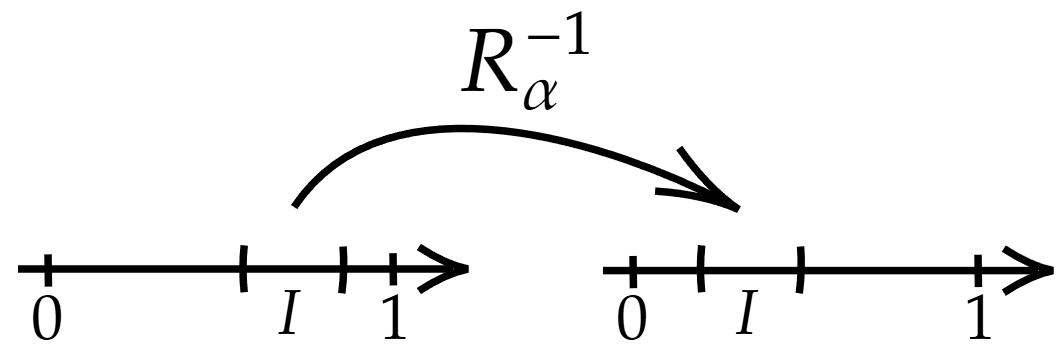
\includegraphics[width = 0.35\textwidth]{fig/2.2.png}
            \captionof{figure}{$R_\alpha$保持测度}
        \end{figure}
        \vspace{-0.5 em}
        如果$I$左端点的值小于$\alpha$，那么$R^{-1}_\alpha(I)$会被分为两个部分，但其测度不会发生变化.\par
        \item 
        \begin{minipage}[t]{0.70\textwidth}
            \wideline
            定义$\setjot[-6]\begin{aligned}[t]
            T_2:\;[0,1) &\to [0,1) \\
            x &\mapsto 2x \mod 1 
        \end{aligned}$\par
        其中$\mcal{B}=\mathrm{Borel}\,\sigmaalg$，$m=m_\mathrm{Leb}$为Lebesgue测度.\par
        可以证明：$m_\mathrm{Leb}\left(T^{-1}_2(I)\right)=m_\mathrm{Leb}(I)$，因此$T_2$为$[0,1)$上的一个保测映射.\par
        右图直观地展示了为何$T_2$可以保持半代数的测度.\par
        更一般地，对于$\forall k\in\mbb{N},T_k(x)=k\cdot x\mod 1$是$[0,1)$上的保测映射.
        \end{minipage}
        \begin{minipage}[t]{0.25\textwidth}
            \vspace{-1em}
            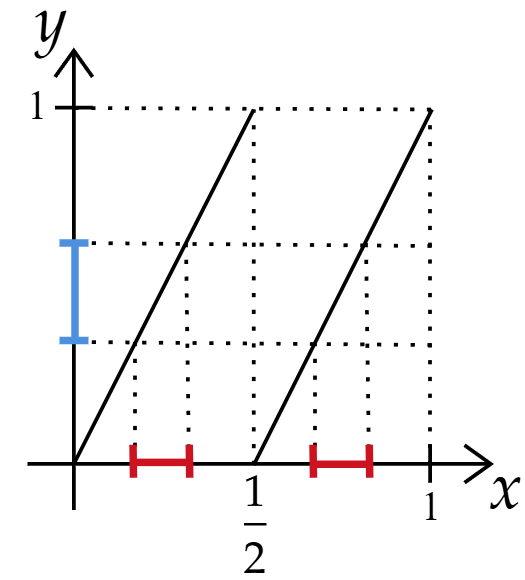
\includegraphics[width=1\textwidth]{fig/2.3.png}
            \captionof{figure}{$T_2$保持测度}
        \end{minipage}
        \item 
        \begin{minipage}[t]{0.65\textwidth}
            \wideline
            下一个例子是高斯映射，定义为：
            {\setjot[-6]\begin{align*}
                T:(0,1) &\to (0,1) \\
                x &\mapsto \frac{1}{x} \mod 1
            \end{align*}}
            $\mcal{B}$为$(0,1)$上的Borel$\,\sigmaalg$，概率测度使用如下微分和积分定义：
            \begin{align*}
                \d m(x)=\frac{1}{\ln{2}}\frac{1}{1+x}\d x 
                \Leftrightarrow \forall\, A\in\mcal{B},m(A)=\frac{1}{\ln 2}\int_A{\frac{1}{1+x}}\d x
            \end{align*}
            下一步，证明$T$是一个保测映射.\par
        \end{minipage}
        \begin{minipage}[t]{0.3\textwidth}
            \vspace{-1.5em}
            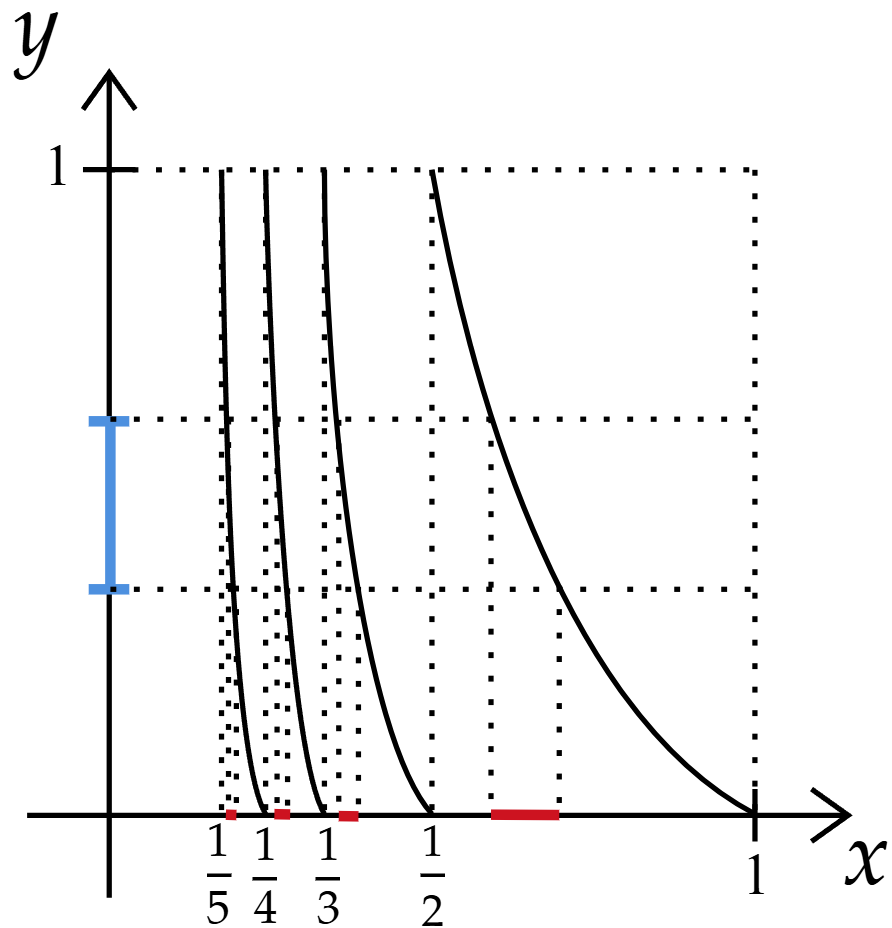
\includegraphics[width=1\textwidth]{fig/2.4.png}
            \captionof{figure}{高斯映射保持测度}
        \end{minipage}
        高斯映射的图象如右图所示，可以看出高斯映射由可数条曲线组成，在自右向左第$k$根曲线上高斯映射可以写成：$\setjot[-6]\begin{aligned}
            T^k_2: \left(\frac{1}{k+1},\frac{1}{k}\right) &\to (0,1) \\
            x &\mapsto \frac{1}{x} \mod 1 = \frac{1}{x} - k
        \end{aligned}$.\par
        对于$\forall\, I=(a,b)\subseteq (0,1) ,(T^k_2)^{-1}(I)=\left(\frac{1}{b+k},\frac{1}{a+k}\right)\Rightarrow T^{-1}_2(I) = \bigcup_{k\in\mbb{N}}\left(\frac{1}{b+k},\frac{1}{a+k}\right)$，则
        {\setjot[-1]\begin{align*}
            m \left(T^{-1}_2(I)\right) &= \sum_{k=1}^\infty{\frac{1}{\ln 2}\int_{\frac{1}{b+k}}^{\frac{1}{a+k}}{\frac{1}{1+x}\d x}}=\sum_{k=1}^\infty \left(\frac{1}{\ln{2}}\left(\ln\frac{a+N+1}{a+1}-\ln{\frac{b+N+1}{b+1}}\right)\right) \\
            &=\lim_{N\to\infty}\sum_{k=1}^N\left(\frac{1}{\ln{2}}\left(\ln\frac{a+N+1}{a+1}-\ln{\frac{b+N+1}{b+1}}\right)\right) \\  
            &= \lim_{N\to\infty}\left(\frac{1}{\ln{2}}\left(\ln\frac{a+N+1}{a+1}-\ln\frac{b+N+1}{b+1}\right)\right) \\&
            = \lim_{N\to\infty}\left(\frac{1}{\ln{2}}\left(\ln\frac{a+N+1}{b+N+1}-\ln\frac{b+1}{a+1}\right)\right) \\
            &= \frac{1}{\ln{2}}\left(\ln\frac{b+1}{a+1}\right)=\frac{1}{\ln{2}}\int_a^b{\frac{1}{1+x}}\d x = m(I).
        \end{align*}}
        \item 最后是一个积概率空间的例子.设$Y=\{1,2,\cdots,n\},\mcal{B}_Y=\{Y\text{的所有子集}\},\setjot[-6]\begin{aligned}[t]
            m_Y: \mcal{B}_Y &\to [0,1] \\
            A &\mapsto \frac{|A|}{n}
        \end{aligned}$.\par
        设$X=\prod_{i=-\infty}^\infty{Y}=\left\{(\cdots,x_{-1},x_0,x_1,\cdots)|x_i\in Y\right\}$，其上的$\sigmaalg$和概率测度参考定义$\ref{def:1.10}$、定义$\ref{def:1.11}$和定义$\ref{def:1.12}$.\par
        定义$Y$上的左位移映射
        {\setjot[-3]\begin{align*}
            T: X&\to X \\
            (\cdots,-x_2,-x_1,x_0,x_1,x_2,\cdots) &\mapsto (\cdots,x_{-1},x_0,x_1,x_2,x_3,\cdots) 
        \end{align*}}
        \begin{itemize}
            \item $T$是保测映射，称为\bluebf{Bernouli转移}.\par
            $T$是可测映射，这是因为$T^{-1}\mcal{S}=\mcal{S} \Rightarrow T^{-1}\mcal{B}_x\subseteq \mcal{B}_x$.
            \item $\forall\, E=\cdots\times Y\times A_m\times\cdots\times A_n\times Y\times\cdots\in\mcal{S}$，\par
            知$T^{-1}E=\cdots\times Y\times Y\times A_m\times\cdots\times A_{n-1}\times A_n\times Y\times \cdots$\par
            由积概率测度的定义可知$m(E)=m(T^{-1}E)$.
        \end{itemize}
    \end{enumerate}
\end{instance}




\section{遍历映射}

\begin{definition}{遍历映射}
    设$(X,\mcal{B},m)$为概率测度空间，$T:X\to X$为保测映射，如果$T$满足$\forall\, B\in\mcal{B},T^{-1}B=B \Rightarrow m(B)=0\text{或}1$，那么称$T$是\textbf{遍历映射}.
\end{definition}

下面的例子利用$R_\alpha$构造了一个遍历映射.
\begin{instance}
    设$\setjot[-6]\begin{aligned}[t]
        R_\alpha:[0,1) &\to [0,1) \\
        x &\mapsto x+\alpha \mod 1 
    \end{aligned}$，其中$\alpha=\frac{n}{m}\in\mbb{Q},m\geq 1$，$m,n$互素.\par
    $\forall\, x\in [0,1)$，定义$\delta_x(A)=\begin{cases}
        1, & x\in A \\
        0, & x\notin A
    \end{cases}$，其中$A\in\mcal{B}$，称上述定义为支在点$x$处的\bluebf{Dirac测度}.\par
    可以证明$\delta_x$是$\left([0,1),\mcal{B}\right)$上的一个概率测度.\par
    令$\mu = \frac{1}{m}\sum_{i=0}^{m-1}{\delta_{\tfrac{i}{m}}}$，它实际上就是分别支在$m$个均匀分布在$[0,1)$上的点的Dirac测度的平均值，因此也可以证明$\mu$是$\left([0,1),\mcal{B}\right)$上的一个概率测度.\par
    由于$R_\alpha(x)=x+\frac{n}{m}\mod 1$，因此$R_\alpha$作用在$\mathrm{supp}(\mu)=\left\{0,\frac{1}{m},\cdots,\frac{m-1}{m}\right\}$上为支集中点的轮换，因此有$\frac{1}{m}\sum_{i=0}^{m-1}{\delta_{R_\alpha \left(\tfrac{i}{m}\right)}(A)}=\frac{1}{m}\sum_{i=0}^{m-1}{\delta_{\tfrac{i}{m}}(A)}$.\par
    又因为$\delta_{R_\alpha \left(\tfrac{i}{m}\right)}(A)=\delta_{\tfrac{i}{m}}(R_\alpha^{-1}(A))$，得
    $$\mu(R_\alpha^{-1}(A))=\frac{1}{m}\sum_{i=0}^{m-1}{\delta_{\tfrac{i}{m}}(R_\alpha^{-1}(A))}=\frac{1}{m}\sum_{i=0}^{m-1}{\delta_{R_\alpha \left(\tfrac{i}{m}\right)}(A)}=\frac{1}{m}\sum_{i=0}^{m-1}{\delta_{\tfrac{i}{m}}(A)}=\mu(A)$$
    这说明$R_\alpha:\left([0,1),\mcal{B},\mu \right)\to\left([0,1),\mcal{B},\mu \right)$是保测映射.\par
    下面证明$R_\alpha$是遍历映射.\par
    对$\forall A\in\mcal{B},R_\alpha^{-1}(A)=A$，可分两种情况：
    \begin{enumerate}
        \item 若$A\cap\mathrm{supp}(\mu)=\varnothing$，则有$\mu(A)=0$.
        \item 若$A\cap\mathrm{supp}(\mu)\neq\varnothing$，由于$R_\alpha$保持$\mathrm{supp(\mu)}$，所以$R_\alpha(A)=A$.\par
        设$x_0\in A\cap\mathrm{supp}(\mu),x_0=\frac{j}{m}$，则$R_\alpha^k(x_0)=\frac{j}{m}+\frac{n}{m}\cdot k (\mod 1)$.\par
        因为$m,n$互素$\Rightarrow A\supseteq \left\{R_\alpha^k(x_0)|k\in\mbb{Z}\right\} = \mathrm{supp}(\mu)$.\par
        $\Rightarrow \mu(A)=1$
    \end{enumerate}
\end{instance}

遍历映射的另一个意义是，如果一个映射是保测映射但并非遍历映射，那么就可以把测度空间分解为两个不交的子集，在每个子集定义保测映射.对于遍历映射，我们就不能这么做.\par
设$T:(X,\mcal{B},m)\to(X,\mcal{B},m)$是保测映射，如果$\exists\, B\in\mcal{B}$，使得$0<m(B)<1,T^{-1}B=B$，那么就可以在$B$和$X\setminus B$上定义新的保测映射，也就是：
{\setjot[-3]\begin{align*}
    &\qquad T|_B:B\to B  & &\;\; T|_{X\setminus B}:X\setminus B\to X\setminus B \\
    &\text{关于}m_B(A)=\frac{m(A)}{m(B)} & &\text{关于}m_{X\setminus B}(A)=\frac{m(A)}{m(X\setminus B)} \\
    &\text{是保测映射}(\forall\, A\in B) & &\text{是保测映射}(\forall\, A\in X\setminus B)
\end{align*}}

遍历性有若干形式的等价条件，下面两个定理分别从集合和函数的角度给出了两组描述方式.
\begin{theorem}{遍历映射的等价条件}\label{thm:2.4}
    \wideline
    设$(X,\mcal{B},m)$是一个概率测度空间，$T:(X,\mcal{B},m)\to(X,\mcal{B},m)$是保测映射，则以下结论等价：
    \begin{enumerate}[(1)]
        \item $T$是一个保测遍历映射
        \item $\forall\, B\in\mcal{B}$，$m \left(T^{-1}B\triangle B\right)=0 \Rightarrow m(B)=0\text{或}1$
        \item $\forall\, A\in\mcal{B},m(A)>0 \Rightarrow m \left(\bigcup_{i=1}^\infty{T^{-i}A}\right)=1$
        \item $\forall\, A,B\in\mcal{B},m(A)>0,m(B)>0,\exists\,n\in\mbb{N}$，使得$m \left(T^{-n}A\cap B\right)>0$
    \end{enumerate}
\end{theorem}
\begin{proof}
    $(1)\Rightarrow(2)$：令$E=\bigcap_{n=1}^\infty{\left(\bigcup_{i=n}^\infty{T^{-i}B}\right)}$.
    \begin{itemize}
        \item $T^{-1}E=E$.\par
        令$A_n=\bigcup_{i=n}^\infty{T^{-i}B}$，则$A_0\supseteq A_1\supseteq \cdots\supseteq A_n\supseteq A_{n+1}\supseteq \cdots$，且$T^{-1}A_n=A_{n+1}$.\par
        $T^{-1}(E)=T^{-1}\left(\bigcap_{n=1}^\infty{A_n}\right)=\bigcap_{n=1}^\infty{T^{-1}A_n}=\bigcap_{n=2}^\infty{T^{-1}A_n}=\bigcap_{n=1}^\infty{A_n}=E$.\par
        由遍历映射的定义可得$m(E)=0$或$1$.
        \item 由$T$为保测映射，所以$m \left(T^{-1}B\triangle B=0\right)\Rightarrow m \left(T^{-2}B\triangle T^{-1}B\right)=m \left(T^{-1}\left(T^{-1}B\triangle B\right)\right)=0$.\par
        依此类推可得$m \left(T^{-(k+1)}B\triangle T^{-k}B\right)=0,\forall k\in\mbb{N}$.\par
        这表明$B,T^{-1}B,T^{-2}B,\cdots,T^{-k}B,\cdots$中任意两个集合之间只相差1个零测集.\par
        因此$\forall\, A_n,m \left(A_n\triangle B\right)=0\Rightarrow m(E\triangle B=0)\Rightarrow m(B)=m(E)=0$或$1$.
    \end{itemize}\par
    $(2)\Rightarrow (3)$：$\forall\, A\in\mcal{B},m(A)>0$，令$E=\bigcup_{n=1}^\infty{T^{-n}A}$.\par
    $T^{-1}E=\bigcup_{n=1}^{\infty}T^{-(n+1)}A=\bigcup_{n=2}^\infty{T^{-n}A}\subseteq E$.\par
    又由于$m(E)=m(T^{-1}E) \Rightarrow m(T^{-1}E\triangle E)=0 \xLongrightarrow{\text{条件}(2)} m(E)=0$或$1$.\par
    而$m(E)=m \left(T^{-1}\left(\bigcup_{n=0}^\infty{T^{-n}A}\right)\right)=m \left(\bigcup_{n=0}^\infty{T^{-n}A}\right)\geq m(A) >0$.\par
    因此$m \left(\bigcup_{i=1}^\infty{T^{-i}A}\right)=1$.\par
    $(3)\Rightarrow(4)$：$\forall\, A,B\in\mcal{B},m(A)>0,m(B)>0$，由(3)可知$m \left(\bigcup_{n=1}^\infty{T^{-n}A}\right)=1$.\par
    所以$m\left(B\cap \bigcup_{i=1}^\infty{T^{-i}A}\right)=m\left(\bigcup_{n=1}^\infty{\left(B\cap T^{-n}A\right)}\right)\xlongequal{\text{可列可加性}}\sum_{n=1}^\infty{m\left(B\cap T^{-n}A\right)}>0$.\par
    $\Rightarrow \exists\, n\in\mbb{N},m\left(T^{-n}A \cap B\right)>0$.\par
    $(4)\Rightarrow(1)$：设$B\in\mcal{B},T^{-1}B=B$，如果$m(B)\in(0,1)$，那么令$A=X\setminus B$，有$m(A)>0$.\par
    $T^{-1}A=T^{-1}(X\setminus B)=T^{-1}X\setminus T^{-1}B = X\setminus B=A\ \Rightarrow T^{-n}A=A$，\par
    $\Rightarrow \forall\, n\in\mbb{N},m(T^{-n}A\cap B)=m(A\cap B)=m \left((X\setminus B)\cap B\right) =0$.与(4)矛盾!
\end{proof}



\begin{theorem}{遍历映射的等价函数刻画}
    \wideline
    设$(X,\mcal{B},m)$是一个概率测度空间，$T:(X,\mcal{B},m)\to(X,\mcal{B},m)$是保测映射，则以下结论等价：
    \begin{enumerate}[(1)]
        \item $T$是一个保测遍历映射
        \item $\forall\, f:X\to\mbb{C}$是可测函数，若$f\circ T=f\aew$，那么$f=\mathrm{const}\aew$
        \item $\forall\, f\in L^2(X,\mcal{B},m)$，如果$f\circ T=f\aew$，那么$f=\mathrm{const}\aew$
    \end{enumerate}
\end{theorem}
\begin{proof}
    $(2)\Rightarrow(3)$：由平方可积函数定义可得.\par
    $(3)\Rightarrow(1)$：设$B\in\mcal{B},T^{-1}B=B$，考虑$f=\chi_B\in L^2(X,\mcal{B},m)$.\par
    $\Rightarrow \chi_{T^{-1}B}=\chi_B \Rightarrow \chi_{B}\circ T=\chi_B \Rightarrow \chi_B=c \aew$\par
    因为$\chi_B$是特征函数，故$c=0$或$1\Rightarrow m(B)=\int\chi_B\d m=0$或$1$.\par
    $(1)\Rightarrow (2)$：设$f:X\to\mbb{C}$满足$f\circ T=f\aew$.\par
    设存在$S\subseteq X,m(S)=0$使得$f(Tx)=f(x),\forall x\in X\setminus S$.\par
    令$E_c=\{x\in X|f(x)\geq c\}(\forall\, c\in\mbb{R})$.\par
    $\forall\, y\in T^{-1}E_c\setminus S,f(y)=f(Ty)\geq c\Rightarrow y\in E_c$.\par
    因此$T^{-1}E_c\setminus S\subseteq E_c$，由保测映射$m(T^{-1}E_c)=m(E_c)\Rightarrow m(T^{-1}E_c\triangle E_c=0)$.\par
    由定理$\ref{thm:2.4}(2)$可得$m(E_c)=0$或$1$.从而可以找到$g=c$，使得$f$上所有点几乎处处在$g=c$上，进而$f=c\aew.$\par
\end{proof}







